\section{Results}

\subsection{NMF decomposes high-dimensional data into a small number of components}

\begin{figure}
\centering
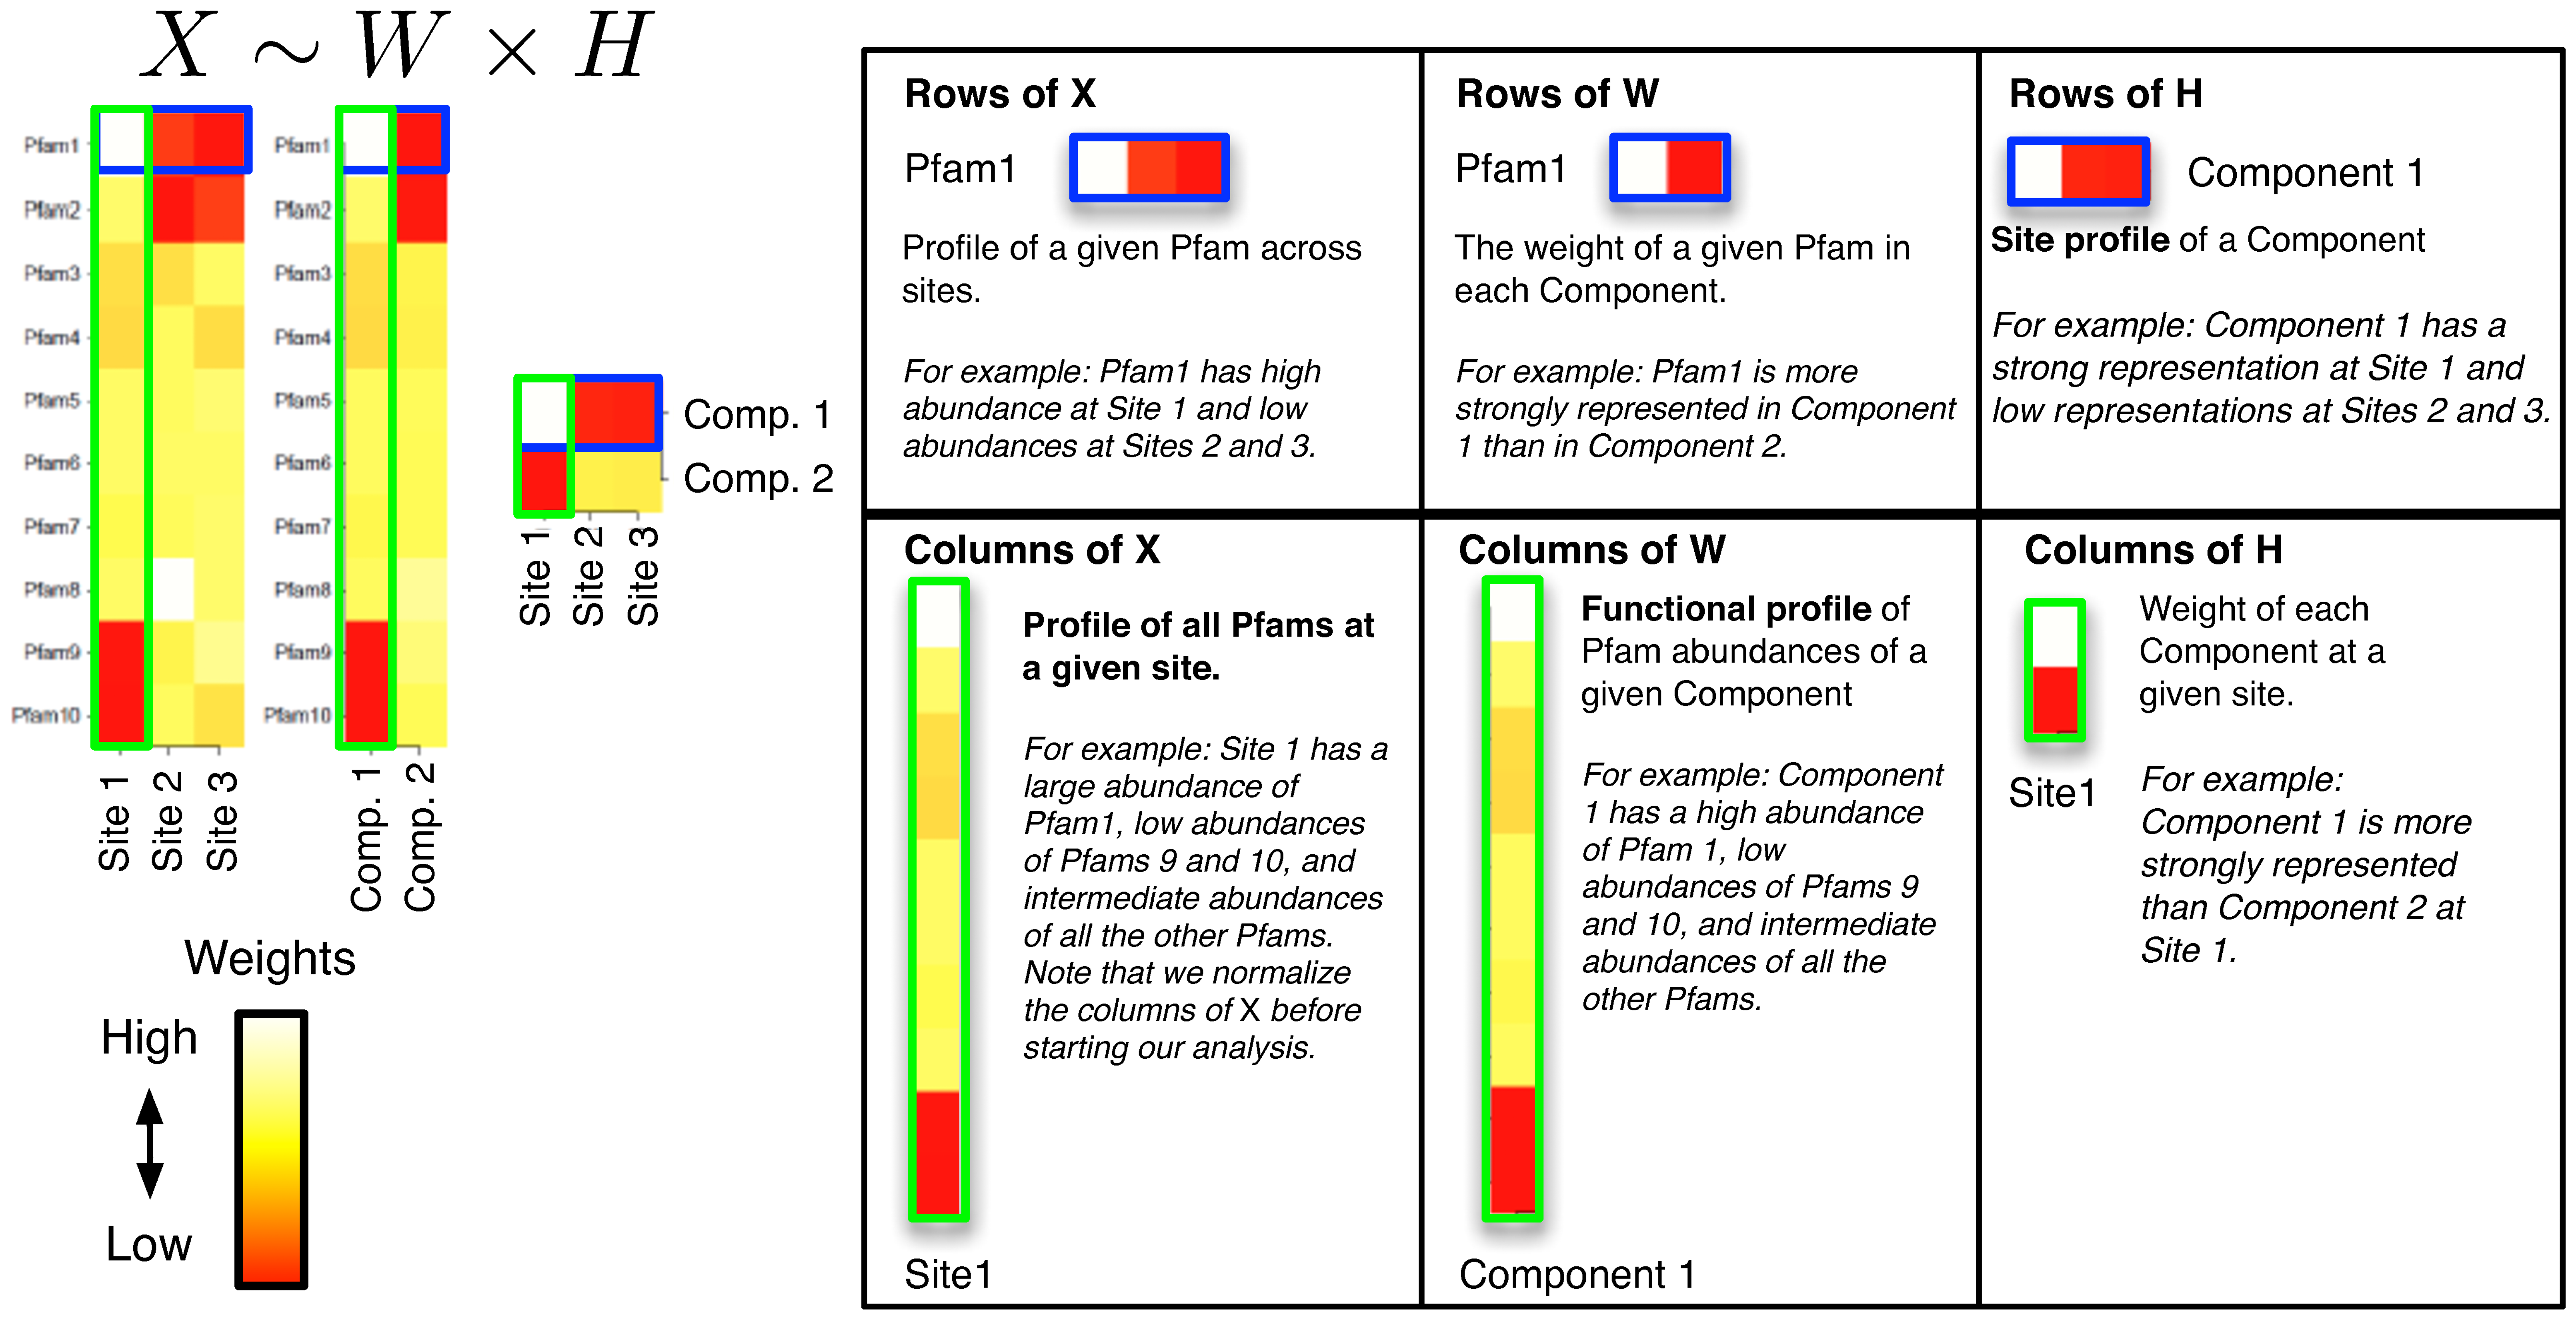
\includegraphics[width=\textwidth]{NMF/figures/fig1}
\caption{\textbf{A conceptual illustration of NMF decomposition.} Left: We start with a sample of $p=10$ Pfams across $s=3$ sites, and perform a rank $k=2$ factorization, $X\approx WH$. In real applications the reduction in rank is more dramatic. Color codes show Pfam relative abundance. Right: The subfigures illustrate different ways of looking at the decomposition using rows and columns.}
\label{NMF_fig1}
\end{figure}

We selected a subset of 45 out of a total of 79 GOS samples to avoid known problems involving contamination and outliers (see Materials and Methods).  Our selection criteria were similar to those used in other studies \cite{gianoulis_quantifying_2009, patel_analysis_2010, raes_toward_2011}. These 45 samples represent a wide geographic and environmental range (Table S7). We then made Pfam assignments for all proteins found in the 45 samples, counted the Pfam assignments for each sample, and normalized these counts by the total number of assignments in the sample (see Materials and Methods). The end result is a ``profile matrix'' with 45 columns representing the samples and 8214 rows representing Pfams. This profile matrix gives the estimated relative abundance of Pfams in each site and is the starting point for NMF decomposition. 

The NMF decomposition can be thought of as an empirical attempt to describe observed Pfam patterns in terms of a small number of functional ``components" (see Figure \ref{NMF_fig1}).  Each component is associated with a ``functional profile" describing the average relative abundance of each Pfam in the component, and with a ``site profile", describing how strongly the component is represented at each site.  Thus, the observed Pfam distribution at a site is approximated as a weighted sum of the functional profiles of our components, with each component's profile weighted by its site profile at that site. In explicit terms, we approximate the observed $p\times s$ Pfam read matrix ($X$) as the product of: a $p\times k$ matrix whose $k$ columns are functional profiles for our components ($W$); and a $k\times s$ matrix whose $k$ rows are the corresponding site profiles ($H$). The demonstrative example in Figure \ref{NMF_fig1}, uses a factorization of rank 2 ($k$) to reduce a $10\times 3$ matrix of Pfam abundances ($X$) into $10\times 2$ matrix of functional profiles ($W$) and a $2\times 3$ matrix of site profiles ($H$). In this example, the best approximation found by NMF has one component with a functional profile very similar to that of the first site, and one that is similar to the remaining two sites.

We applied a concordance method (see Materials and Methods and \cite{jiang_non-negative_2012}) to compare possible decomposition ranks, and found that 5 is a suitable rank for the NMF decomposition of the GOS data (Figure \ref{ModelSelection}). This means that the observed Pfam profile matrix ($8214 \times 45$) can be stably approximated using 5 functional profiles and associated site profiles. 

\subsection{Identifying and interpreting the biological basis of functional profiles of components}

\begin{figure}
\centering
% \subfigure[]{\includegraphics[scale=0.5, trim=0mm 0mm 55mm 13mm, clip=TRUE]{subplots_random.Rout-3.pdf}}
% \subfigure[]{\includegraphics[scale=0.5, trim=5mm 0mm 0mm 10mm, clip=TRUE]{GOS/subplots_random.Rout-1.pdf}} 
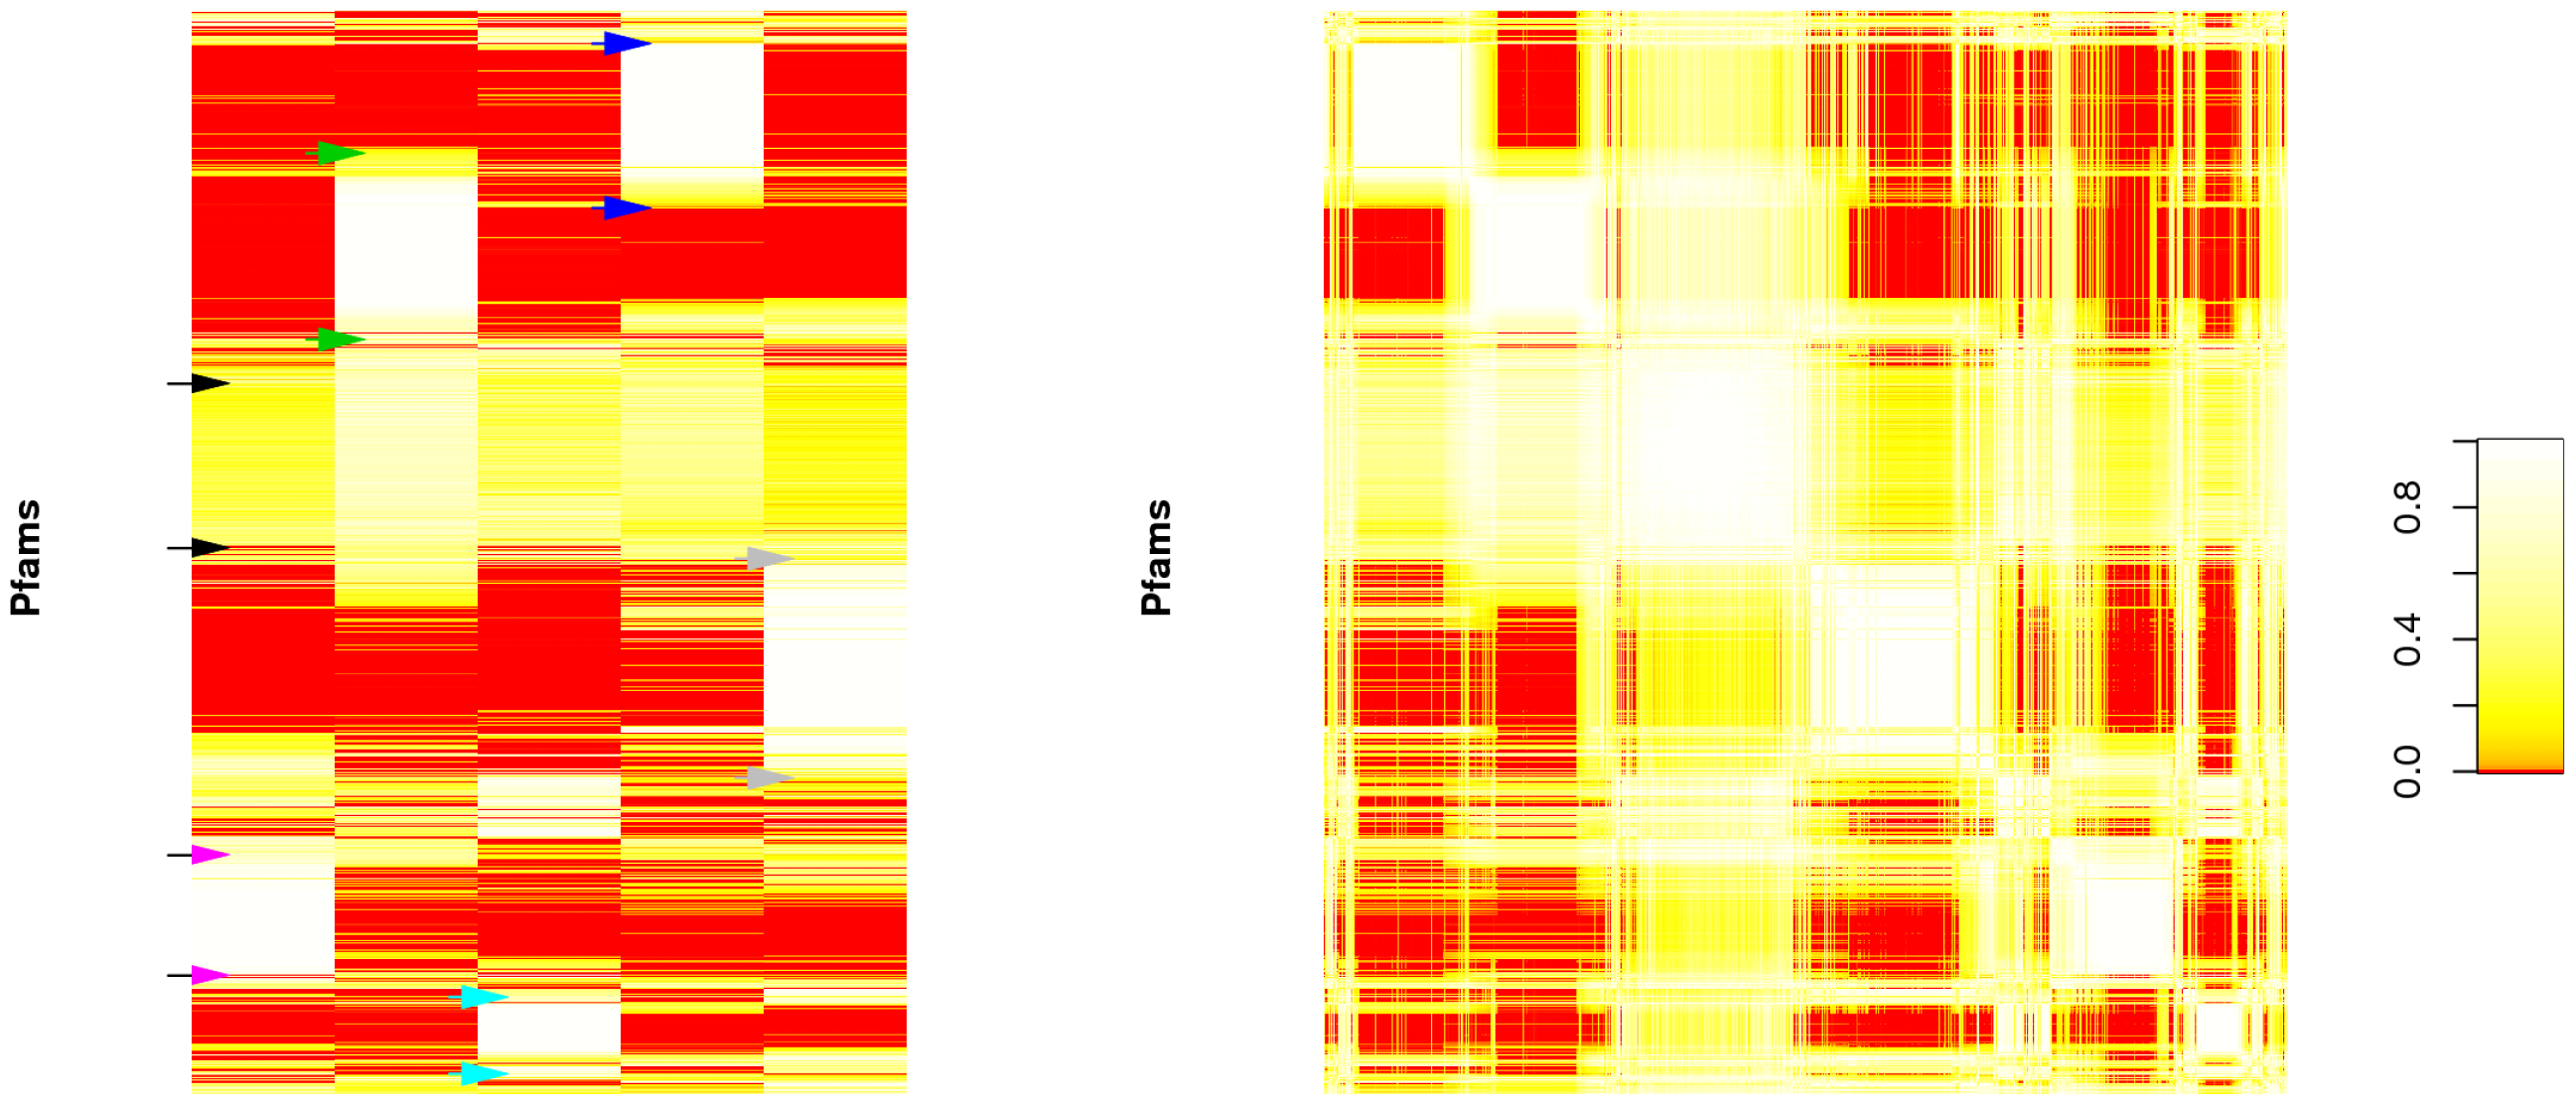
\includegraphics[width=\textwidth]{NMF/figures/fig2}
\caption[]{\textbf{Functional profiles of NMF generated components and the corresponding similarity matrix.} a) Five ecological components identified by using NMF across Pfam functional profiles (rows). Colored arrows roughly indicate the clusters of ``characteristic'' Pfams corresponding to each of the five components; black arrows roughly indicate the cluster of ``ubiquitous'' Pfams. b) Pfam profile similarity matrices generated using NMF filtering. The matrices are aligned so that the same row corresponds to the same Pfam in each matrix. Pfams with similar profiles are grouped by applying spectral reordering to the similarity matrix (see Materials and Methods). Due to visualization and computational limitations, a random subset of 1000 Pfams are used for ordering and display.}
\label{W}
\end{figure}

The functional profiles for each of our five components are shown in Figure \ref{W}a.  Each component has one or more sets of ``characteristic'' Pfams, which have relatively high abundance within that component and low abundance in other components (see blocks labelled by arrows in Figure \ref{W}a). However, unlike some traditional clustering approaches, NMF does not restrict Pfams to be assigned to a single component, and in fact some Pfams are found in high concentration in multiple components. For example, Figure \ref{W}a shows areas of overlap occurring on the same row between the large blocks of high concentration near the top of components 2 and 4 (the blocks indicated by blue and green arrows in Figure \ref{W}a).

We then constructed a Pfam similarity matrix, using NMF as a \emph{filter} (Figure \ref{W}b). This filtered similarity matrix shows clearer patterns of clustering than we find using ``direct" similarity or PCA-based filtering (Figure \ref{PfamSimilarity}). These clusters naturally overlap in many cases, illustrating the advantages of not relying on a strict clustering algorithm. Most of the clusters in the similarity matrix correspond to Pfam blocks dominated by a single component, as can be seen by comparing with Figure \ref{W}a. However, the third cluster instead corresponds to Pfams that are broadly distributed across all of the components.  This can be seen by comparison with Figure \ref{W}a (the Pfam block indicated by black arrows), or by the mid-intensity cross that encompasses the white core of the cluster in in Figure \ref{W}b.

To better understand the functional relevance of the NMF components, we identified Pfams that were strongly associated with each component.  \new{We applied NMF on the whole Pfam profile} and we selected Pfams based on the \emph{correlation} between their spatial distribution and the site profile of each component (Figure \ref{H}a).  We contend that this correlation-based approach is preferable to ``specificity-" \cite{jiang_non-negative_2012} or ``projection-" \cite{carmona2006biclustering, kim_sparse_2007} based methods, because it avoids undue bias toward either rare or ubiquitous Pfams (see Materials and Methods and Figure \ref{specComp}).

We found that some of our components had a suite of strongly associated Pfams whose distribution across sites was strongly correlated with the site profile of the component. Component 2 had the clearest group of strongly associated Pfams (126 Pfams have a correlation $> 0.8$ to this component).  Components 1 and 5 also had groups of Pfams with relatively high correlation values (28 and 52 Pfams have a correlation $> 0.8$ to component 1 and 5 respectively), while Components 3 and 4 did not have any strongly associated Pfams (Figure \ref{simHist}). 

To determine if there are particular functions that are associated with each of the components, we manually inspected the lists of Pfams that were most strongly correlated with their respective component. Interestingly, we found commonality in the functional annotation of Pfams associated with components that had strongly associated Pfams (i.e., Components 1, 2, and 5) (Table S1, S2 and S5). Using the 100 most strongly associated Pfams for each component, we found that 40\% of the Pfams with known function were related to transport and signalling in Component 1 (which we call ``Signalling") (Table S1); 37\% of the Pfams with known function were photosystem-associated in Component 2 (``Photosystem"); and 22\% of the Pfams with known function were phage-associated in Component 5 (``Phage") (See Table S5). In Components 3 and 4, which did not have strongly associated Pfams (Tables S3, S4), we could not identify any functional patterns.  Components 3 and 4 may represent combinations of different ecological components that are not separated in this particular decomposition. 

The proportion of Pfams without any annotations ranged from 15\% (Component 4) to 54\% (Component 2: Photosystem). Unidentified Pfams with high association to Components 1, 2 and 5 may have similar functional themes to other Pfams seen in these components, or they may have functions that are ecologically linked to the identified theme, or they may be associated taxonomically rather than functionally (ie., they may be expressed by the same taxa that express the identified Pfams).  In the future, we suggest developing statistical methods to identify groups of strong associations, and associated false discovery rates.

Additionally, we inspected the Pfams that were associated with the ``ubiquitous" cluster previously identified in \ref{W}. Many of these Pfams are associated with bacterial primary metabolism and only 1\% of these had unknown functions (Table S6). This is a striking difference compared to the 15--54\% proportion of unknown Pfams seen in the five NMF components. 

\subsection{Characterizing the site profiles of components}

\begin{figure}
\centering
%\includegraphics[trim=5mm 22mm 0mm 10mm, clip=TRUE, scale=1.3]{nsd2.pdf}
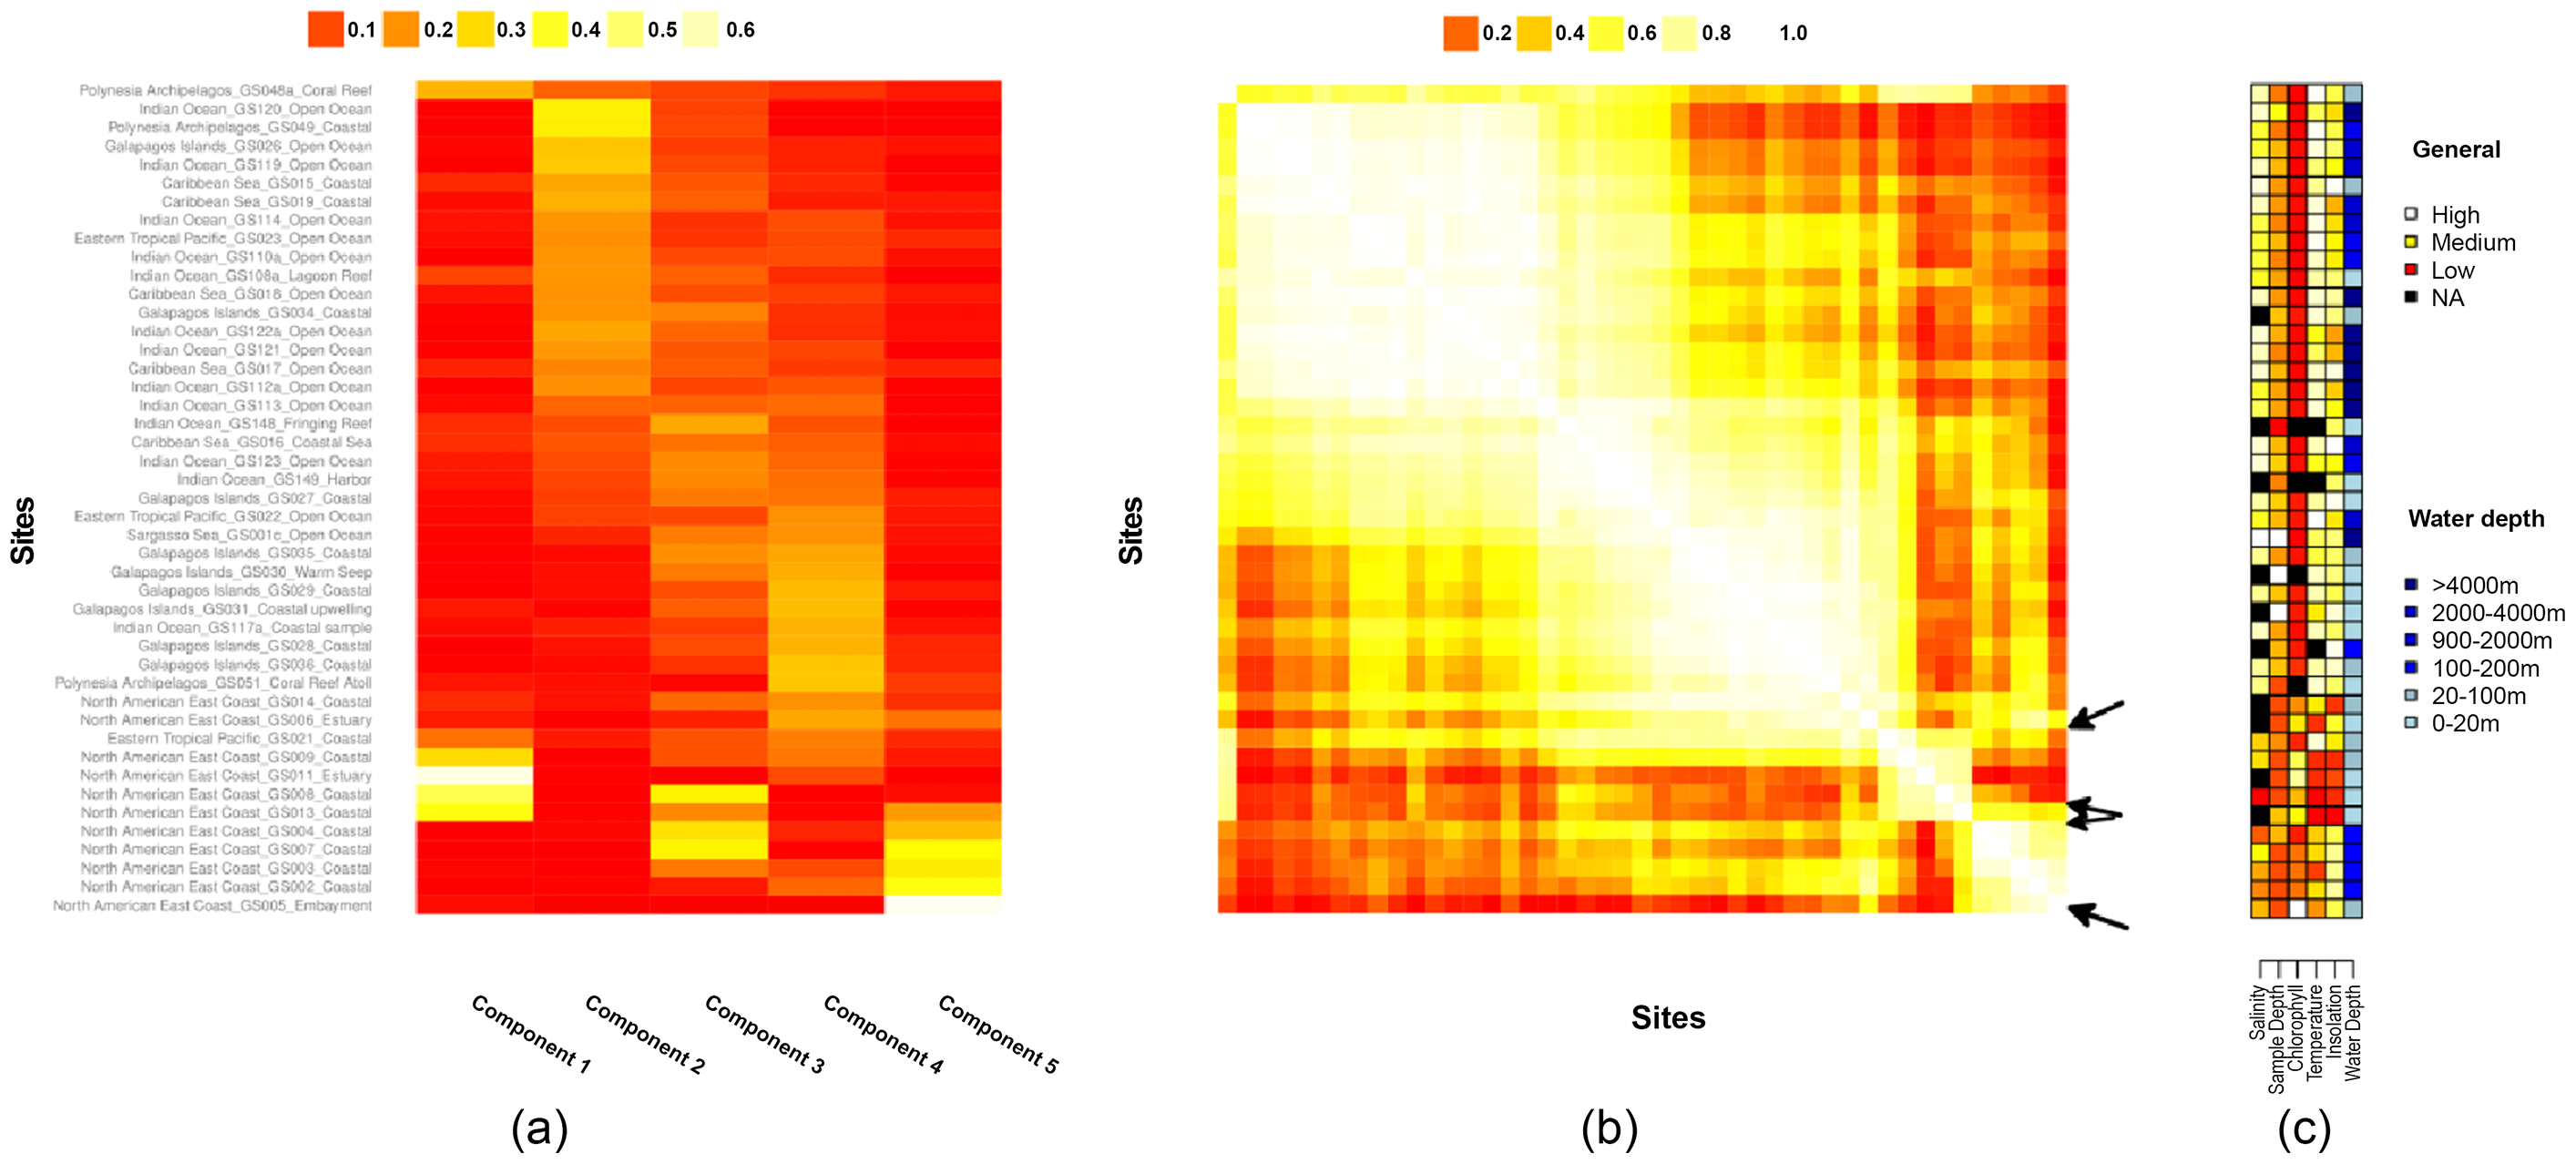
\includegraphics[width=\textwidth]{NMF/figures/fig3}
\caption{\textbf{Components across sites.} a) Weight for each of the five components at each of the 45 sites ($H^T$);  b) the site-similarity matrix ($\hat H^T \hat H$); c) environmental variables for the sites.  The matrices are aligned so that the same row corresponds to the same site in each matrix.  Sites are ordered by applying spectral reordering to the similarity matrix (see Materials and Methods). Rows are aligned across the three matrices.}
\label{H} 
\end{figure}

Figure \ref{H}a shows the estimated site profile for each of the five components.  Components 2 (Photosystem) and 4 (Unidentified) are broadly distributed;  Components 1 (Signalling) and 5 (Phage) are largely restricted to a handful of sites; and component 3 (Unidentified) shows an intermediate pattern.  There is a great deal of overlap between site profiles for different components. \new{For example, component 3 has relatively high similarity to components 2 and 4 (0.57 and 0.65 respectively, see \ref{component_sim} for a similarity heatmap among components).}  

Figure \ref{H}b shows the pattern of filtered similarity between sites.  We see clear patterns of grouping, which do not emerge when we calculate functional distances without filtering, or use PCA rather than NMF filtering (Figure \ref{SimilarityCompare}). As with the Pfams, we see clusters roughly associated with our components, but there is more overlap than with the Pfam clusters (\ref{W}b).

Figure \ref{H}c shows the distribution of environmental variables measured at each site.  Inspection of Figure \ref{H} reveals qualitative correspondence between environmental factors and clusters of similar sites in the similarity matrix. For example, the ``North American East Coast" samples are divided into two groups in the bottom right of the similarity matrix (see Figure \ref{H}b). Inspection of the environmental features suggests that the split in these samples also corresponds with differences in insolation and water depth. 

%\subsection{Components}

We can also examine patterns of similarity between the components themselves, using site profiles or functional profiles (see Figure \ref{component_sim}). All five components have strikingly high similarities in their functional profiles, indicating a lot of Pfams which are well represented in many components. Similarity in site profiles is much lower on average, indicating that many pairs of components do not tend to overlap within samples. Overall patterns of similarity also differ: for example, the Phage component (5) and Signalling component (1) have a very high level of functional similarity, but very low similarity in their site profiles.